% Figure 3(b): vector artwork at natural size (321pt x 164pt).
% All numbers are from Table 2; no hand-scaled raster data.
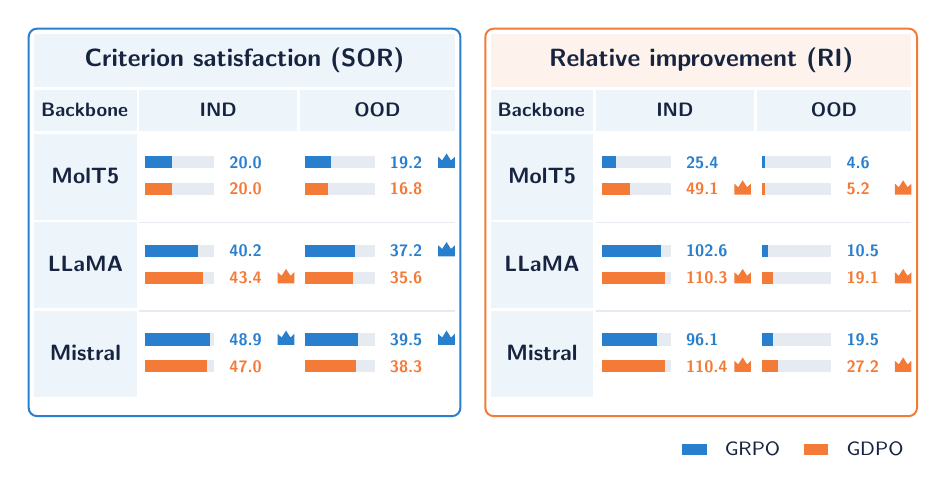
\begin{tikzpicture}[x=1pt,y=1pt,baseline=(current bounding box.south),
every node/.style={font=\sffamily\fontsize{6.7}{7.8}\selectfont}]
\definecolor{cmB}{HTML}{287FCD}
\definecolor{cmO}{HTML}{F47A37}
\definecolor{cmGrey}{HTML}{E6EBF1}
\definecolor{cmInk}{HTML}{172440}
\definecolor{cmPaleBlue}{HTML}{EDF5FB}
\definecolor{cmPaleOrange}{HTML}{FDF3EC}
\draw[cmB,line width=.72pt,rounded corners=3pt] (0,22) rectangle (156,162);
\fill[cmPaleBlue] (2,141) rectangle (154,160);
\node[anchor=center,font=\sffamily\bfseries\fontsize{9.2}{10}\selectfont,text=cmInk] at (78,150.4) {Criterion satisfaction (SOR)};
\fill[cmPaleBlue] (2,125) rectangle (39,140);
\node[font=\sffamily\bfseries\fontsize{6.6}{7.3}\selectfont,text=cmInk] at (20.2,132.8) {Backbone};
\fill[cmPaleBlue] (40,125) rectangle (97,140);
\node[font=\sffamily\bfseries\fontsize{7}{8}\selectfont,text=cmInk] at (68.5,132.8) {IND};
\fill[cmPaleBlue] (98,125) rectangle (154,140);
\node[font=\sffamily\bfseries\fontsize{7}{8}\selectfont,text=cmInk] at (126,132.8) {OOD};
\fill[cmPaleBlue] (2,93) rectangle (39,124);
\node[font=\sffamily\bfseries\fontsize{8}{9}\selectfont,text=cmInk] at (20.5,109) {MolT5};
\draw[cmGrey,line width=.55pt] (40,92) -- (154,92);
\fill[cmGrey] (42,111.5) rectangle (67,115.9);
\fill[cmB] (42,111.5) rectangle (51.62,115.9);
\node[anchor=west,text=cmB,font=\sffamily\bfseries\fontsize{6.4}{7.1}\selectfont] at (69,113.7) {20.0};
\fill[cmGrey] (42,101.8) rectangle (67,106.2);
\fill[cmO] (42,101.8) rectangle (51.62,106.2);
\node[anchor=west,text=cmO,font=\sffamily\bfseries\fontsize{6.4}{7.1}\selectfont] at (69,104.0) {20.0};
\fill[cmGrey] (100,111.5) rectangle (125,115.9);
\fill[cmB] (100,111.5) rectangle (109.23,115.9);
\node[anchor=west,text=cmB,font=\sffamily\bfseries\fontsize{6.4}{7.1}\selectfont] at (127,113.7) {19.2};
\fill[cmB] (148,111.7) -- (148,115.7) -- (149.4,114.4) -- (151,116.9) -- (152.6,114.4) -- (154,115.7) -- (154,111.7) -- cycle;
\fill[cmGrey] (100,101.8) rectangle (125,106.2);
\fill[cmO] (100,101.8) rectangle (108.08,106.2);
\node[anchor=west,text=cmO,font=\sffamily\bfseries\fontsize{6.4}{7.1}\selectfont] at (127,104.0) {16.8};
\fill[cmPaleBlue] (2,61) rectangle (39,92);
\node[font=\sffamily\bfseries\fontsize{8}{9}\selectfont,text=cmInk] at (20.5,77) {LLaMA};
\draw[cmGrey,line width=.55pt] (40,60) -- (154,60);
\fill[cmGrey] (42,79.5) rectangle (67,83.9);
\fill[cmB] (42,79.5) rectangle (61.33,83.9);
\node[anchor=west,text=cmB,font=\sffamily\bfseries\fontsize{6.4}{7.1}\selectfont] at (69,81.7) {40.2};
\fill[cmGrey] (42,69.8) rectangle (67,74.2);
\fill[cmO] (42,69.8) rectangle (62.87,74.2);
\node[anchor=west,text=cmO,font=\sffamily\bfseries\fontsize{6.4}{7.1}\selectfont] at (69,72.0) {43.4};
\fill[cmO] (90,70) -- (90,74) -- (91.4,72.7) -- (93,75.2) -- (94.6,72.7) -- (96,74) -- (96,70) -- cycle;
\fill[cmGrey] (100,79.5) rectangle (125,83.9);
\fill[cmB] (100,79.5) rectangle (117.88,83.9);
\node[anchor=west,text=cmB,font=\sffamily\bfseries\fontsize{6.4}{7.1}\selectfont] at (127,81.7) {37.2};
\fill[cmB] (148,79.7) -- (148,83.7) -- (149.4,82.4) -- (151,84.9) -- (152.6,82.4) -- (154,83.7) -- (154,79.7) -- cycle;
\fill[cmGrey] (100,69.8) rectangle (125,74.2);
\fill[cmO] (100,69.8) rectangle (117.12,74.2);
\node[anchor=west,text=cmO,font=\sffamily\bfseries\fontsize{6.4}{7.1}\selectfont] at (127,72.0) {35.6};
\fill[cmPaleBlue] (2,29) rectangle (39,60);
\node[font=\sffamily\bfseries\fontsize{8}{9}\selectfont,text=cmInk] at (20.5,45) {Mistral};
\fill[cmGrey] (42,47.5) rectangle (67,51.9);
\fill[cmB] (42,47.5) rectangle (65.51,51.9);
\node[anchor=west,text=cmB,font=\sffamily\bfseries\fontsize{6.4}{7.1}\selectfont] at (69,49.7) {48.9};
\fill[cmB] (90,47.7) -- (90,51.7) -- (91.4,50.400000000000006) -- (93,52.900000000000006) -- (94.6,50.400000000000006) -- (96,51.7) -- (96,47.7) -- cycle;
\fill[cmGrey] (42,37.8) rectangle (67,42.2);
\fill[cmO] (42,37.8) rectangle (64.60,42.2);
\node[anchor=west,text=cmO,font=\sffamily\bfseries\fontsize{6.4}{7.1}\selectfont] at (69,40.0) {47.0};
\fill[cmGrey] (100,47.5) rectangle (125,51.9);
\fill[cmB] (100,47.5) rectangle (118.99,51.9);
\node[anchor=west,text=cmB,font=\sffamily\bfseries\fontsize{6.4}{7.1}\selectfont] at (127,49.7) {39.5};
\fill[cmB] (148,47.7) -- (148,51.7) -- (149.4,50.400000000000006) -- (151,52.900000000000006) -- (152.6,50.400000000000006) -- (154,51.7) -- (154,47.7) -- cycle;
\fill[cmGrey] (100,37.8) rectangle (125,42.2);
\fill[cmO] (100,37.8) rectangle (118.41,42.2);
\node[anchor=west,text=cmO,font=\sffamily\bfseries\fontsize{6.4}{7.1}\selectfont] at (127,40.0) {38.3};
\draw[cmO,line width=.72pt,rounded corners=3pt] (165,22) rectangle (321,162);
\fill[cmPaleOrange] (167,141) rectangle (319,160);
\node[anchor=center,font=\sffamily\bfseries\fontsize{9.2}{10}\selectfont,text=cmInk] at (243,150.4) {Relative improvement (RI)};
\fill[cmPaleBlue] (167,125) rectangle (204,140);
\node[font=\sffamily\bfseries\fontsize{6.6}{7.3}\selectfont,text=cmInk] at (185.2,132.8) {Backbone};
\fill[cmPaleBlue] (205,125) rectangle (262,140);
\node[font=\sffamily\bfseries\fontsize{7}{8}\selectfont,text=cmInk] at (233.5,132.8) {IND};
\fill[cmPaleBlue] (263,125) rectangle (319,140);
\node[font=\sffamily\bfseries\fontsize{7}{8}\selectfont,text=cmInk] at (291,132.8) {OOD};
\fill[cmPaleBlue] (167,93) rectangle (204,124);
\node[font=\sffamily\bfseries\fontsize{8}{9}\selectfont,text=cmInk] at (185.5,109) {MolT5};
\draw[cmGrey,line width=.55pt] (205,92) -- (319,92);
\fill[cmGrey] (207,111.5) rectangle (232,115.9);
\fill[cmB] (207,111.5) rectangle (212.29,115.9);
\node[anchor=west,text=cmB,font=\sffamily\bfseries\fontsize{6.4}{7.1}\selectfont] at (234,113.7) {25.4};
\fill[cmGrey] (207,101.8) rectangle (232,106.2);
\fill[cmO] (207,101.8) rectangle (217.23,106.2);
\node[anchor=west,text=cmO,font=\sffamily\bfseries\fontsize{6.4}{7.1}\selectfont] at (234,104.0) {49.1};
\fill[cmO] (255,102) -- (255,106) -- (256.4,104.7) -- (258,107.2) -- (259.6,104.7) -- (261,106) -- (261,102) -- cycle;
\fill[cmGrey] (265,111.5) rectangle (290,115.9);
\fill[cmB] (265,111.5) rectangle (265.96,115.9);
\node[anchor=west,text=cmB,font=\sffamily\bfseries\fontsize{6.4}{7.1}\selectfont] at (292,113.7) {4.6};
\fill[cmGrey] (265,101.8) rectangle (290,106.2);
\fill[cmO] (265,101.8) rectangle (266.08,106.2);
\node[anchor=west,text=cmO,font=\sffamily\bfseries\fontsize{6.4}{7.1}\selectfont] at (292,104.0) {5.2};
\fill[cmO] (313,102) -- (313,106) -- (314.4,104.7) -- (316,107.2) -- (317.6,104.7) -- (319,106) -- (319,102) -- cycle;
\fill[cmPaleBlue] (167,61) rectangle (204,92);
\node[font=\sffamily\bfseries\fontsize{8}{9}\selectfont,text=cmInk] at (185.5,77) {LLaMA};
\draw[cmGrey,line width=.55pt] (205,60) -- (319,60);
\fill[cmGrey] (207,79.5) rectangle (232,83.9);
\fill[cmB] (207,79.5) rectangle (228.38,83.9);
\node[anchor=west,text=cmB,font=\sffamily\bfseries\fontsize{6.4}{7.1}\selectfont] at (234,81.7) {102.6};
\fill[cmGrey] (207,69.8) rectangle (232,74.2);
\fill[cmO] (207,69.8) rectangle (229.98,74.2);
\node[anchor=west,text=cmO,font=\sffamily\bfseries\fontsize{6.4}{7.1}\selectfont] at (234,72.0) {110.3};
\fill[cmO] (255,70) -- (255,74) -- (256.4,72.7) -- (258,75.2) -- (259.6,72.7) -- (261,74) -- (261,70) -- cycle;
\fill[cmGrey] (265,79.5) rectangle (290,83.9);
\fill[cmB] (265,79.5) rectangle (267.19,83.9);
\node[anchor=west,text=cmB,font=\sffamily\bfseries\fontsize{6.4}{7.1}\selectfont] at (292,81.7) {10.5};
\fill[cmGrey] (265,69.8) rectangle (290,74.2);
\fill[cmO] (265,69.8) rectangle (268.98,74.2);
\node[anchor=west,text=cmO,font=\sffamily\bfseries\fontsize{6.4}{7.1}\selectfont] at (292,72.0) {19.1};
\fill[cmO] (313,70) -- (313,74) -- (314.4,72.7) -- (316,75.2) -- (317.6,72.7) -- (319,74) -- (319,70) -- cycle;
\fill[cmPaleBlue] (167,29) rectangle (204,60);
\node[font=\sffamily\bfseries\fontsize{8}{9}\selectfont,text=cmInk] at (185.5,45) {Mistral};
\fill[cmGrey] (207,47.5) rectangle (232,51.9);
\fill[cmB] (207,47.5) rectangle (227.02,51.9);
\node[anchor=west,text=cmB,font=\sffamily\bfseries\fontsize{6.4}{7.1}\selectfont] at (234,49.7) {96.1};
\fill[cmGrey] (207,37.8) rectangle (232,42.2);
\fill[cmO] (207,37.8) rectangle (230.00,42.2);
\node[anchor=west,text=cmO,font=\sffamily\bfseries\fontsize{6.4}{7.1}\selectfont] at (234,40.0) {110.4};
\fill[cmO] (255,38) -- (255,42) -- (256.4,40.7) -- (258,43.2) -- (259.6,40.7) -- (261,42) -- (261,38) -- cycle;
\fill[cmGrey] (265,47.5) rectangle (290,51.9);
\fill[cmB] (265,47.5) rectangle (269.06,51.9);
\node[anchor=west,text=cmB,font=\sffamily\bfseries\fontsize{6.4}{7.1}\selectfont] at (292,49.7) {19.5};
\fill[cmGrey] (265,37.8) rectangle (290,42.2);
\fill[cmO] (265,37.8) rectangle (270.67,42.2);
\node[anchor=west,text=cmO,font=\sffamily\bfseries\fontsize{6.4}{7.1}\selectfont] at (292,40.0) {27.2};
\fill[cmO] (313,38) -- (313,42) -- (314.4,40.7) -- (316,43.2) -- (317.6,40.7) -- (319,42) -- (319,38) -- cycle;
\fill[cmB] (236,8) rectangle (245,12);
\node[anchor=west,font=\sffamily\fontsize{7}{8}\selectfont,text=cmInk] at (248,10.2) {GRPO};
\fill[cmO] (280,8) rectangle (289,12);
\node[anchor=west,font=\sffamily\fontsize{7}{8}\selectfont,text=cmInk] at (292,10.2) {GDPO};
\end{tikzpicture}
